\label{sec:eval}

\begin{figure*}[htbp]
\centering
\label{fig:overhead}
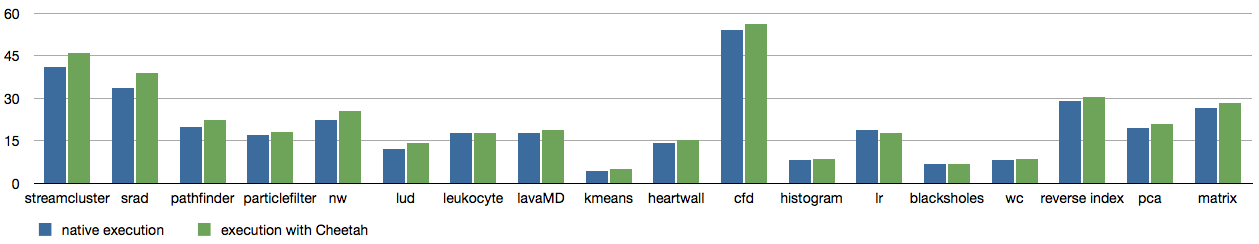
\includegraphics[width=2\columnwidth]{figure/overhead}
\caption{Runtime overhead incurred by \Cheetah{}. All Rodinia benchmarks are run with 48 threads, while all Phoenix benchmarks are run with 16 threads. We exclude any benchmark with small execution time. The time is averaged on three executions.}
\end{figure*}

We evaluate \cheetah{} on an AMD Opteron Magny-Cours machine, which has 48 1.6 GHz cores and 128 GB memory. We test multithreaded programs from two well-known benchmark suites: Phoenix~\cite{} and Rodinia~\cite{}. These benchmarks cover popular threading models, such as pthread~\cite{} and OpenMP~\cite{}. Table~\ref{} shows the detailed description of each benchmark. We use gcc 4.6 to compile these benchmarks with {\tt -O2} option. For Phoenix benchmarks, we run them with 16 threads because these benchmarks often have small working sets. For Rodinia benchmarks, we run them with 48 threads. As \cheetah is based sampling, a benchmark should run long enough (at least 5 second) to get enough statistical samples. Otherwise, the code complete quickly and no one cares about the false sharing. 

For \cheetah{}, we configure with instruction-based sampling at a sampling period of 64K instructions (sample one instruction for every 64K instructions). Figure~\ref{} shows the runtime overhead incurred by \cheetah{}. From the figure, we can see that \cheetah{} incurs low runtime overhead, less than 3\% on average. Moreover, \cheetah{} identifies two false sharing problems in two benchmarks: Pheonix Linear\_Regression and Rodinia StreamCluster. In the remaining of this section, we discuss these two benchmarks separately: we verify the false sharing code and evaluate the accuracy of the assessment of optimization potentials. Finally, we study the false sharing that \cheetah{} does not detect in these benchmarks and verify that they have negligible impact to the overall program execution. 

\subsection{Linear\_Regression}
Figure~\ref{fig:lr} shows the output of \cheetah{}, which points out that array {\tt tid\_args} with the structure type {\tt lreg\_args} incurs a severe false sharing problem. The reason for this is that ...

To address the problem, we pad the structure {\tt lreg\_args} with extra bytes to force all threads to access different cache lines. The optimization lead to a 5.7$\times$ speedup, which exactly matches the assessment 5.76$\times$ given by \cheetah{}.

\begin{figure}
\begin{minipage}{\columnwidth}

\centering

\fbox
{
\begin{minipage}{3in}
FALSE SHARING: start 0x400004b8 end 0x400044b8 (with size 4000). Accesses 1263 invalidations 27f writes 501 total latency on this object was 102988 cycles.
Latency information: totalThreads 16 totalThreadsAccesses 12e1 totalThreadsCycles 106389 longestRuntime 7652 threadReduceRate 0.164697 totalPossibleImprovementRate 576.172748\% (realRuntime 7738 predictedRuntime 1343)
\end{minipage}
}
\vspace{1em}
\caption{The output of \cheetah{} for Linear\_Regression.}
\label{fig:lr}
\end{minipage}
\end{figure}


\begin{figure}
\begin{verbatim}
tid_args = (lreg_args *)calloc(
	        sizeof(lreg_args), num_procs);

typedef struct
{
    pthread_t tid;
    POINT_T *points;
    int num_elems;
    long long SX;
    long long SY;
    long long SXX;
    long long SYY;
    long long SXY;
} lreg_args;	    
\end{verbatim}
\caption{The data object and the structure type that cause false sharing.}
\label{lr:code}
\end{figure}

\subsection{StreamCluster}

Figure~\ref{fig:sc} shows the output of StreamCluster. It identifies one false sharing. Correlating back to the source code, we find that ..

\begin{figure}
\begin{minipage}{\columnwidth}

\centering

\fbox
{
\begin{minipage}{3in}
FALSE SHARING: start 0x4900b058 end 0x4900b458 (with size 400). Accesses b7 invalidations 30 writes 5e total latency on this object was 18659 cycles.
Latency information: totalThreads 16 totalThreadsAccesses 1058c totalThreadsCycles 3328784 longestRuntime 64453 threadReduceRate 0.994541 totalPossibleImprovementRate 102.11116\% (realRuntime 65441 predictedRuntime 64088)
\end{minipage}
}
\vspace{1em}
\caption{The output of \cheetah{} for StreamCluster.}
\label{fig:sc}
\end{minipage}
\end{figure}


\subsection{Missing False Sharing Problems}

\begin{figure}[htbp]
\centering
\label{fig:fsinfs}
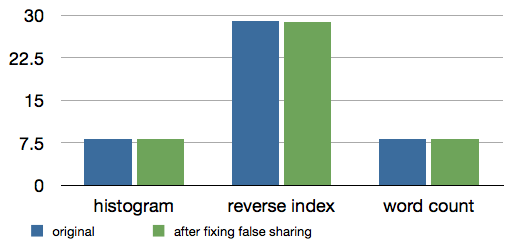
\includegraphics[width=.8\columnwidth]{figure/trivial}
\caption{The false sharing omitted by \cheetah{} has negligible impact to the whole program execution.}
\end{figure}

As we described in Section~\ref{}, \cheetah{} may omit false sharing occurring in the code because of its sampling feature. In this section, we show that the false sharing \cheetah{} misses has negligible performance impact to the whole program execution.  For this purpose, we refer to all the false sharing identified by Predator~\cite{} in both Phoenix and PARSEC benchmarks. These false sharing problems include false sharing occurs in histogram, reverse\_index, and word\_count. Figure~\ref{} shows the performance speedups after we fix all the false sharing. Experimental results show that all these benchmark achieve less than 0.1\%. 

\subsection{Discussions}

\Cheetah{}, with the support of lightweight IBS, can identify cache line false sharing efficiently and effectively. However, its runtime overhead can still be as high as 10-20\%, mainly due to the mechanism of AMD IBS. AMD IBS samples every kind of instructions, including arithmetic instructions (e.g., add, sub, mul, and div) and logic instructions (e.g., comp and test), which are useless for analyzing false sharing. Instead, \cheetah{} only requires sampling memory accesses. Because of this hardware limitation, \cheetah{} needs to filter out useless samples with a software method. Such software method needs \cheetah{} to receive samples and check corresponding bits to test if these samples access memory or not; these processes incur high overhead. Hopefully, the hardware can overcome this limitations in the future by only sampling memory loads and stores.
